%@TheDoctorRAB
%standard white paper/preproposal format
%
%%%%%
%
%REFERENCES
%
%neup.bst - numbered citations in order of appearance, short author list with et al in reference section
%nsf.bst - numbered citations in order of appearance, full author list in references section
%standard.bst - citations with author last name with et al for more than 2 authors; full author list in references section
%ans.bst is for ANS only. 
%
%author = {Lastname, Firstname and Lastname, Firstname and Lastname, Firstname} for all bst formats
%bst renders the author list itself
%
%author = {{Nuclear Regulatory Commission}} if the author is an organization, institution, etc., and not people
%
%title = {{}} for all
%
%for all - use \citep{-} - [1] or (Borrelli, 2021) in the text
%standard.bst \cite{-} - Borrelli (2021) in the text
%standard.bst lists references alphabetically
%the rest list numerically
%
%
%%% slides 
%
%\citep{xxxnna} where the citation should go
%\blfootnote{\fontsize\cite{xxxnna}\fontsize\bibentry{xxxnna}} before \end{frame}
%
%
%%%%%

%%%%% presentation settings
\documentclass[aspectratio=1610,pdftex,dvipsnames,compress,xcolor={dvipsnames}]{beamer}
\usetheme{Boadilla}
\usecolortheme{seahorse}
\beamertemplatenavigationsymbolsempty
\addtobeamertemplate{footnote}{\hskip -2em}{} %pushes footnote to margin
\setbeamerfont{title}{series=\bfseries}
\setbeamertemplate{page number in head/foot}[framenumber] %just gives slide number; comment out for 1/7, 2/7...
\definecolor{BackGround}{RGB}{255,250,240}
\setbeamercolor{background canvas}{bg=BackGround}
%%%%%


%%%%% general 
%\documentclass[11pt,a4paper]{article}
%\usepackage[lmargin=1in,rmargin=1in,tmargin=1in,bmargin=1in]{geometry}
\usepackage[pagewise]{lineno} %line numbering
\usepackage{setspace}
\usepackage{ulem} %strikethrough - do not \sout{\cite{}}
\usepackage{graphicx}
\usepackage{mypythonhighlight,verbatim}
\usepackage{filecontents}
\usepackage{tablefootnote}
\usepackage{footnotehyper}
\usepackage{float}
%\usepackage{subfig}
\usepackage[yyyymmdd]{datetime} %date format
\renewcommand{\dateseparator}{.}
\graphicspath{{img/}} %path to graphics
\setcounter{secnumdepth}{5} %set subsection to nth level
\usepackage{needspace}
\usepackage[stable,hang,flushmargin]{footmisc} %footnotes in section titles and no indent; standard.bst
\usepackage[inline]{enumitem}
\setlist[itemize]{label=\textbullet}
\usepackage{boldline}
\usepackage{makecell}
\usepackage{booktabs}
\usepackage{amssymb}
\usepackage{gensymb}
\usepackage{amsmath,nicefrac}
\usepackage{physics}
\usepackage{lscape}
\usepackage{array}
\usepackage{chngcntr}
\usepackage{hyperref}
\hypersetup{colorlinks,linkcolor=black,citecolor=black,urlcolor=blue} 
%\usepackage{sectsty}
\usepackage{textcomp}
\usepackage{lastpage}
\usepackage{xargs} %for \newcommandx
\usepackage[colorinlistoftodos,prependcaption,textsize=tiny]{todonotes} %makes colored boxes for commenting
\usepackage{soul}
\usepackage{color}
\usepackage{marginnote}
\usepackage[figure,table]{totalcount}
\usepackage[capitalise]{cleveref}
\usepackage{microtype} %improves typography for pdf
\usepackage[pdftex,dvipsnames]{colortbl} %change font color
%%%%%


%%%%% tikz
\usepackage{pgf}
\usepackage{tikz} % required for drawing custom shapes
\usetikzlibrary{shapes,arrows,automata,trees}
%%%%%


%%%%% fonts
\usepackage{times}
%\renewcommand{\sfdefault}{ubuntu}
%arial - uncomment next two lines
%\usepackage{helvet}
%\renewcommand{\familydefault}{\sfdefault}
%%%%%


%%%%% references
%\usepackage[round,semicolon]{natbib} %for (Borrelli 2021; Clooney 2019) - standard.bst 
\usepackage[numbers,sort&compress]{natbib} %for [1-3] - nsf.bst, neup.bst
\setlength{\bibsep}{7pt} %sets space between references
%\renewcommand{\bibsection}{} %suppresses large 'references' heading
%\renewcommand\bibpreamble{\vspace{\baselineskip}} %sets spacing after heading if not using default references heading
%%%%%


%%%%% tables and figures
\usepackage{longtable} %need to put label at top under caption then \\ - use spacing
\usepackage{tablefootnote}
\usepackage{tabularx}
\usepackage{multirow}
\usepackage{tabto} %general tabbed spacing
\usepackage{pdfpages}
\usepackage{wrapfig} %wraps figures around text
\setlength{\intextsep}{0.00mm}
\setlength{\columnsep}{1.00mm}
\usepackage[singlelinecheck=false,labelfont=bf]{caption}
\usepackage{subcaption}
\captionsetup[table]{justification=justified,skip=5pt,labelformat={default},labelsep=period,name={Table}} %sets a space after table caption
\captionsetup[figure]{justification=justified,skip=5pt,labelformat={default},labelsep=period,name={Figure}} %sets space above caption, 'figure' format
\captionsetup[wrapfigure]{justification=centering,aboveskip=0pt,belowskip=0pt,labelformat={default},labelsep=period,name={Fig.}} %sets space above caption, 'figure' format
\captionsetup[wraptable]{justification=centering,aboveskip=0pt,belowskip=0pt,labelformat={default},labelsep=period,name={Table}} %sets space above caption, 'figure' format
%%%%%


%%%%% watermark
%\usepackage[firstpage,vpos=0.63\paperheight]{draftwatermark}
%\SetWatermarkText{\shortstack{DRAFT\\do not distribute}}
%\SetWatermarkScale{0.20}
%%%%%


%%%%% cross referencing files
%\usepackage{xr} %for revisions - will cross reference from one file to here
%\externaldocument{/path/to/auxfilename} %aux file needed
%%%%%


%%%%% toc and glossaries
\usepackage[toc,title]{appendix}
\usepackage[acronym,nomain,nonumberlist]{glossaries}
\makenoidxglossaries
%\usepackage{titlesec,titletoc}
%\renewcommand{\thepart}{ARTICLE \Roman{part}} %puts the label into the command so \thelabel will carry through
%\renewcommand{\thesection}{\arabic{section}} %puts the label into the command so \thelabel will carry through
%\titleformat{\part}{\normalfont\large\bfseries}{\thepart}{}{}[]
%\titlespacing*\part{0pt}{0.95\baselineskip}{0.75\baselineskip}
%\titleformat{\section}[runin]{\normalfont\large\bfseries}{\thesection}{-1em}{}[.]
%\titlespacing*\section{0pt}{0.65\baselineskip}{0.55\baselineskip}
%\titleformat{\subsection}[runin]{\normalfont\normalsize\bfseries}{\thesubsection}{-1em}{}[.]
%\titlespacing*\subsection{0pt}{0.50\baselineskip}{0.35\baselineskip}
%\titleformat{\paragraph}[runin]{\normalfont\normalsize\bfseries\itshape}{\theparagraph}{-1em}{}[.]
%\titlespacing*\paragraph{0pt}{0.45\baselineskip}{0.25\baselineskip}
%\titleformat{\subparagraph}[runin]{\normalfont\normalsize\itshape}{\thesubparagraph}{-1em}{}[.]
%\titlespacing*\subparagraph{0pt}{0.40\baselineskip}{0.25\baselineskip}
%\titleformat{\paragraph}[hang]{\normalfont\normalsize\bfseries}{\theparagraph}{5pt}{}[]
%\titlespacing*\paragraph{0pt}{0.50\baselineskip}{0.25\baselineskip}
%\titleformat{\subparagraph}[runin]{\normalfont\normalsize\itshape}{\thesubparagraph}{-1em}{}[.]
%\titlespacing*\subparagraph{0pt}{0.40\baselineskip}{0.20\baselineskip}
%%%%%


%%%%% editing
\newcommand{\edit}[1]{\textcolor{blue}{#1}} %shortcut for changing font color on revised text
\newcommand{\fn}[1]{\footnote{#1}} %shortcut for footnote tag
\newcommand*\sq{\mathbin{\vcenter{\hbox{\rule{.3ex}{.3ex}}}}} %makes a small square as a separator $\sq$
%\newcommand{\sk}[1]{\sout{#1}} %shortcut for default strikethrough - do not sk through citep
\newcommand\sk{\bgroup\markoverwith{\textcolor{red}{\rule[0.5ex]{1pt}{1pt}}}\ULon} %strikethrough with red line; not in \section{}
%\st{} does strikethrough using soul package but does not like acronyms
\newcommand{\blucell}{\cellcolor{aliceblue}} %use to shade in table cell
\newcommand{\grycekk}{\cellcolor{lightgray}} %use to shade in table cell
\newcommand{\whicell}{\cellcolor{antiquewhite}} %use to shade in table cell
%%%%%


%%%%% colors
%http://latexcolor.com/
%https://en.wikibooks.org/wiki/LaTeX/Colors#:~:text=black%2C%20blue%2C%20brown%2C%20cyan,be%20available%20on%20all%20systems.
\definecolor{aliceblue}{rgb}{0.94, 0.97, 1.0}
\definecolor{antiquewhite}{rgb}{0.98, 0.92, 0.84}
\definecolor{lightmauve}{rgb}{0.86, 0.82, 1.0}
\definecolor{brilliantlavender}{rgb}{0.96, 0.73, 1.0}
\definecolor{brandeisblue}{rgb}{0.0, 0.44, 1.0}
\definecolor{darkmidnightblue}{rgb}{0.0, 0.2, 0.4}

\newcommand{\x}{\cellcolor{aliceblue}} %use to shade in table cell
\newcommand{\y}{\cellcolor{lightgray}} %use to shade in table cell
\newcommand{\z}{\cellcolor{antiquewhite}} %use to shade in table cell
%%%%%


%%%%% acronyms
\newcommand{\acf}{\acrfull} %full acronym
\newcommand{\acl}{\acrlong} %long acronym
\newcommand{\acs}{\acrshort} %short acronym

\newcommand{\acfp}{\acrfullpl} %full acronym plural
\newcommand{\aclp}{\acrlongpl} %long acronym plural
\newcommand{\acsp}{\acrshortpl} %short acronym plural
%%%%%


%%%%% todonotes
\newcommandx{\cmt}[2][1=]{\todo[author=\textbf{STRUCTURE},tickmarkheight=0.15cm,linecolor=red,backgroundcolor=red!25,bordercolor=black,#1]{#2}}
\newcommandx{\con}[2][1=]{\todo[author=\textbf{CONTENT},tickmarkheight=0.15cm,linecolor=brilliantlavender,backgroundcolor=brilliantlavender,bordercolor=black,#1]{#2}}
\newcommandx{\rab}[2][1=]{\todo[noline,author=\textbf{RAB},backgroundcolor=Plum!25,bordercolor=black,#1]{#2}}


%\newcommandx{\jon}[2][1=]{\todo[noline,author=\textbf{ATTN: Johnson},backgroundcolor=blue!25,bordercolor=black,#1]{#2}}
%\newcommandx{\han}[2][1=]{\todo[noline,author=\textbf{ATTN: Haney},backgroundcolor=OliveGreen!25,bordercolor=black,#1]{#2}}
%\newcommandx{\rab}[2][1=]{\todo[author=\textbf{RAB},tickmarkheight=0.15cm,linecolor=Plum,backgroundcolor=Plum!25,bordercolor=black,#1]{#2}}
%\newcommandx{\han}[2][1=]{\todo[author=\textbf{ATTN: Haney},tickmarkheight=0.15cm,linecolor=OliveGreen,backgroundcolor=OliveGreen!25,bordercolor=OliveGreen,#1]{#2}}
%\newcommandx{\jon}[2][1=]{\todo[author=\textbf{ATTN: Johnson},tickmarkheight=0.15cm,linecolor=blue,backgroundcolor=blue!25,bordercolor=blue,#1]{#2}}


% highlighting 
\DeclareRobustCommand{\hlc}[1]{{\sethlcolor{LimeGreen}\hl{#1}}}
\makeatletter
    \if@todonotes@disabled
    \newcommand{\hlh}[2]{#1}
    \else
    \newcommand{\hlh}[2]{\han{#2}\hlc{#1}}
    \fi
    \makeatother

\DeclareRobustCommand{\hld}[1]{{\sethlcolor{CornflowerBlue}\hl{#1}}}
\makeatletter
    \if@todonotes@disabled
    \newcommand{\hlj}[2]{#1}
    \else
    \newcommand{\hlj}[2]{\jon{#2}\hld{#1}}
    \fi
    \makeatother

\DeclareRobustCommand{\hlf}[1]{{\sethlcolor{lightmauve}\hl{#1}}}
\makeatletter
    \if@todonotes@disabled
    \newcommand{\hlb}[2]{#1}
    \else
    \newcommand{\hlb}[2]{\rab{#2}\hlf{#1}}
    \fi
    \makeatother
%%%%%


%%%%% table alignments
\newcolumntype{L}[1]{>{\raggedright\let\newline\\\arraybackslash\hspace{0pt}}m{#1}} %uses \raggedright with m,p{} in table column
\newcolumntype{C}[1]{>{\centering\let\newline\\\arraybackslash\hspace{0pt}}m{#1}} %uses \raggedright with m,p{} in table column
\newcolumntype{R}[1]{>{\raggedleft\let\newline\\\arraybackslash\hspace{0pt}}m{#1}} %uses \raggedright with m,p{} in table column
%%%%%


%%%%% table contents
\makeatletter
\renewcommand\tableofcontents{%
    \@starttoc{toc}%
}
\makeatother

\makeatletter
\renewcommand\listoffigures{%
    \@starttoc{lof}%
}
\makeatother

\makeatletter
\renewcommand\listoftables{%
    \@starttoc{lot}%
}
\makeatother

\makeatletter
\newcommand*\ftp{\fontsize{16.5}{17.5}\selectfont}
\makeatother
%%%%%


%%%%% user commands
\newcommand\blfootnote[1]{%
  \begingroup
  \renewcommand\thefootnote{}\footnote{#1}%
  \addtocounter{footnote}{-1}%
  \endgroup
}

\makeatletter
\renewcommand{\@biblabel}[1]{#1.\hfill} %bibliography ordered list has numbers left flush
\makeatother
%%%%%

%%%%% archived section commands - use titlesec
%\makeatletter
%\renewcommand\section{%
%    \@startsection{section}{1}{\z@ }{0.50\baselineskip}{0.25\baselineskip}
%    {\large \normalfont \bfseries}}%

%\makeatletter
%\renewcommand\paragraph{%
%    \@startsection{paragraph}{4}{\z@ }{0.55\baselineskip}{-1em}
%    {\normalfont \normalsize \bfseries}}%

%\makeatletter
%\renewcommand\subparagraph{%
%    \@startsection{subparagraph}{5}{\z@ }{0.40\baselineskip}{-1em}
%    {\normalfont \normalsize \itshape }}%

%\makeatletter
%\renewcommand\subsection{%
%    \@startsection{subsection}{2}{\z@ }{0.45\baselineskip}{0.25\baselineskip}
%    {\large \normalfont \bfseries}}%
%%%%%


%%%%% header and footer
%\usepackage{fancyhdr}
%\pagestyle{fancy}
%\fancyhf{} %move page number to bottom right
%\renewcommand{\headrulewidth}{0pt} %set line thickness in header; uncomment as is to remove line
%\lhead{\scriptsize Name}
%\lhead{\scriptsize PNUCENE-D-22-xxxxx}
%\chead{\scriptsize \textit{PhD White Paper Project Proposal}}
%\rhead{\scriptsize \today}
%\rfoot{\thepage}
%%%%%


%%%%%%% citations
%\begin{filecontents}{references.bib}
%\end{filecontents}
%%%%%%%


%%%%% acronyms
% alphabetical ordering is automated
\newacronym{nrs}{NRHES}{Nuclear Renewable Hybrid Energy System}
\newacronym{ahp}{AHP}{Analytical Hierarchy Process}
\newacronym{inl}{INL}{Idaho National Laboratory}
\newacronym{orl}{ORNL}{Oak Ridge National Laboratory}
\newacronym{anl}{ANL}{Argonne National Laboratory}
\newacronym{npp}{NPP}{Nuclear Power Plant}
\newacronym{smr}{SMR}{Small Modular Reactor}
\newacronym{ump}{UAMPS}{Utah Associated Municipal Power Systems}
\newacronym{nus}{NuScale}{NuScale Power, LLC}
\newacronym{nrc}{NRC}{United States Nuclear Regulatory Commission}
\newacronym{epri}{EPRI}{Electric Power Research Institute}
\newacronym{nerc}{NERC}{North American Electric Reliability Corporation}
\newacronym{ci}{CI}{Consistency Index}
\newacronym{cr}{CR}{Consistency Ratio}
\newacronym{htse}{HTSE}{High Temperature Steam Electrolysis}
\newacronym{lwr}{LWR}{Light Water Reactor}
\newacronym{eia}{EIA}{U.S. Energy Information Administration}
\newacronym{oer}{OER}{Online Educational Resource}
\newacronym{lms}{LMS}{Learning Management System}
\newacronym{cps}{CPS}{Cyber-Physical Systems}
\newacronym{nsf}{NSF}{National Science Foundation}
\newacronym{wsc}{WSC}{Western Services Corporation}
\newacronym{cae}{CAES}{Center for Advanced Energy Studies}
\newacronym{hsl}{HSSL}{Human System Simulation Laboratory}
\newacronym{pwr}{PWR}{Pressurized Water Reactor}
\newacronym{bwr}{BWR}{Boiling Water Reactor}
\newacronym{roi}{ROI}{Return on Investment}
\newacronym{ic}{I\&C}{Instrumentation \& Controls}
\newacronym{mwe}{MWe}{Megawatts-electric}
\newacronym{ics}{ICS}{Industrial Control Systems}
\newacronym{sca}{SCADA}{Supervisory Control and Data Acquisition}
\newacronym{ip}{IP}{Internet Protocol}
\newacronym{udp}{UDP}{User Datagram Protocol}
\newacronym{tva}{TVA}{Tennessee Valley Authority}
\newacronym{plc}{PLC}{Programmable Logic Controller}
\newacronym{vfd}{VFD}{Variable Frequency Drive}
\newacronym{khp}{KHNP}{Korean Hydro \& Nuclear Power Co., Ltd}
\newacronym{onl}{ORNL}{Oak Ridge National Laboratory}
\newacronym{jcp}{JCPOA}{Joint Comprehensive Plan of Action}
\newacronym{mim}{MITM}{Man in the Middle}
\newacronym{dos}{DDoS}{Distributed Denial of Service}
\newacronym{tcp}{TCP/IP}{Transmission Control Protocol/Internet Protocol}
\newacronym{dnp}{DNP3}{Distributed Network Protocol 3}
\newacronym{pra}{PRA}{Probabilistic Risk Assessment}
\newacronym{cs}{CS}{Critical System}
\newacronym{loc}{LOCA}{Loss of Coolant Accident}
\newacronym{hmi}{HMI}{Human Machine Interface}
\newacronym{pha}{PHA}{Preliminary Hazards Analysis}
\newacronym{bol}{BOL}{Beginning-of-Life}
\newacronym{eol}{EOL}{End-of-Life}
\newacronym{mol}{MOL}{Middle-of-Life}
\newacronym{imu}{IMUNES}{Integrated Multiprotocol Network Emulator/Simulator}
\newacronym{ccc}{CCC}{Computing Community Consortium}
\newacronym{neu}{NEUP}{Nuclear Energy University Program}
\newacronym{doe}{DOE}{United States Department of Energy}
\newacronym{nei}{NEI}{Nuclear Energy Institute}
\newacronym{nit}{NITRD}{Networking Information Technology Research \& Development Program}
\newacronym{rcs}{RCS}{Reactor Cooling System}
\newacronym{con}{IC}{Initial Condition}
\newacronym{csi}{CSIS}{Center for Strategic \& International Studies}
\newacronym{pcap}{PCAP}{packet capture file}
\newacronym{dc}{DC}{Direct-Current}
\newacronym{ac}{AC}{Alternating-Current}
\newacronym{iff}{UIIF}{Idaho Falls Center for Higher Education}
\newacronym{snl}{SNL}{Sandia National Laboratory}
\newacronym{cie}{CIE}{Cyber-Informed Engineering}
\newacronym{cds}{CRDS}{Control Rod Drive System}
\newacronym{cdm}{CRDM}{Control Rod Drive Mechanism}
\newacronym{fma}{FMEA}{Failure Modes \& Effects Analysis}
\newacronym{rpn}{RPN}{Risk Priority Number}
\newacronym{scr}{SCR}{silicon controller rectifier}
\newacronym{hvc}{HVAC}{Heating, Ventilation \& Air Conditioning}
\newacronym{ttb}{TTB}{Time-to-Boil}
\newacronym{sis}{SIS}{Safety Instrumented System}
\newacronym{ui}{UI}{University of Idaho}
\newacronym{ala}{ALARA}{As Low As Reasonably Achievable}
\newacronym{pdf}{PDF}{Probability Density Function}
\newacronym{cdf}{CDF}{Cumulative Distribution Function}
%\newacronym{}{}{}
%%%%%

%%%%% spacing
%\onehalfspacing %linespacing
%\setstretch{1.05} %linespacing
%\spacing{1.25} %equivalent to 1.5 line spacing in Word
%%%%%


%%%%% linenumbering
%\linenumbers %toggle line numbers
%\pagewiselinenumbers %reset line numbers on new page
%\modulolinenumbers[1] %line numbering interval
%%%%%


%%%%% title page
\addtocounter{framenumber}{-1} %does not count the title slide in the slide count
\title[NE529 -- Risk Assessment]{NE529\\RISK ASSESSMENT\\Probability \& statistics\\2}
\author[@TheDoctorRAB]{R. A. Borrelli}
\institute[]{
    \acl{ui}\\
    \vspace{0.10in}
    
\includegraphics[width=0.20\textwidth]{ne-logo.png}
    }
\date{\acl{iff}}
%%%%%

\begin{document}


%%%%% title page with no footer
{
    \setbeamertemplate{footline}{}
    \begin{frame}
        \titlepage
    \end{frame}
}
%%%%%


\begin{frame}{Learning objectives}
    \begin{enumerate}[series=outerlist,topsep=0pt,itemsep=15pt,leftmargin=*,label=(\arabic*)]
        \item[]Demonstrating the importance of statistics
        \item[]Explaining the relevance to the field  
        \item[]Analyzing and interpreting data  
        \item[]Deconstructing myths about statistics  
        \item[]Deriving basic metrics
        \item[]Chapter 7 in the book
    \end{enumerate}
\end{frame}


\begin{frame}{Background}
    \begin{enumerate}[series=outerlist,topsep=0pt,itemsep=21pt,leftmargin=*,label=(\arabic*)]
        \item[]Has anyone taken a statistics course?
        \item[]Math classes tend not to focus on engineering so it is annoying
        \item[]Python very useful for statistical analysis
    \end{enumerate}
\end{frame}


\begin{frame}{Learning nodes}
    \begin{columns}[t]

        \begin{column}{0.50\textwidth}
            \begin{enumerate}[series=outerlist,topsep=0pt,itemsep=1pt,leftmargin=*,label=(\arabic*)]
                \item[]\textbf{Probability and statistics definitions}
                    \vspace{0.10in}
                \item[]\textbf{Probability distributions}
                    \vspace{0.10in}
                \item[]\textbf{Likelihood}
                    \vspace{0.10in}
                \item[]\textbf{Statistics critique}
                    \vspace{0.10in}
                \item[]\textbf{Classic case studies}
                \item[]Cholera
                \item[]World War II
                \item[]Challenger
            \end{enumerate}
        \end{column}

        \begin{column}{0.50\textwidth}
            \begin{enumerate}[series=outerlist,topsep=0pt,itemsep=1pt,leftmargin=*,label=(\arabic*)]
                \item[]\hfill\textbf{Misconceptions}
            \end{enumerate}
        \end{column}

    \end{columns}
\end{frame}


\begin{frame}{}
    \begin{figure}
        \centering
        
\includegraphics[width=0.80\textwidth]{zoidberg.jpg}
%        \caption{}
    \end{figure}
\end{frame}


\begin{frame}[plain]{}
    \centering\LARGE\textbf{What is probability?}
\end{frame}


\addtocounter{framenumber}{-1}
\begin{frame}{Probability theory was invented by Pascal and de Fermat for gambling}
    \begin{enumerate}[series=outerlist,topsep=0pt,itemsep=5pt,leftmargin=*,label=(\arabic*)]
        \item[]Counting cards can up your odds in blackjack to almost over 50:50
        \item[]What is the objective of blackjack?
        \item[]Cards 2--6 have a value of +1
        \item[]Cards 7--9 have a value of 0
        \item[]Cards 10-A have a value of -1
        \item[]How are these `probabilities'?
        \item[]Keep a running total = running count
        \item[]Divide by the number of decks = true count
        \item[]When would you want to bet high?
        \item[]In a standard 6 deck blackjack game each true count will move the house edge half a percent toward the player
        \item[]You still need to know how to play though
    \end{enumerate}
\end{frame}


\begin{frame}{Clearly, probability theory is essential for risk assessment}
    \begin{enumerate}[series=outerlist,topsep=0pt,itemsep=21pt,leftmargin=*,label=(\arabic*)]
        \item[]Perception of probability is not necessarily what the real probability is  
        \item[]This was the point of Monty Hall and the modified Russian roulette
        \item[]Risk perception is hugely important
        \item[]Dice is usually a common starting example
        \item[]And we know the expected value of dice
    \end{enumerate}
\end{frame}


\begin{frame}{Craps}
    \begin{enumerate}[series=outerlist,topsep=0pt,itemsep=15pt,leftmargin=*,label=(\arabic*)]
        \item[]\href{http://wizardofodds.com/play/craps/v2/}{Wizard of odds}
        \item[]Off -- Bet `pass' win on 7, 11
        \item[]Point -- Win if point is thrown before craps (2,3,12)
        \item[]Then the `don't' is the opposite
        \item[]There's a whole bunch of other bets: box cars, snake eyes, etc.
        \item[]What is the probability of these?
        \item[]So the reason craps is popular is because there are a lot of favorable probabilities
    \end{enumerate}
\end{frame}


\begin{frame}{Event needs to be \textit{clearly characterized} before deriving probabilities}
    \begin{enumerate}[series=outerlist,topsep=0pt,itemsep=11pt,leftmargin=*,label=(\arabic*)]
        \item[]Wrong probability if describing the wrong event  
        \item[]Wrong assumptions
        \item[]What is an independent event? Dependent event?
    \end{enumerate}

    \vspace{0.25in}

    \begin{enumerate}[series=outerlist,topsep=0pt,itemsep=11pt,leftmargin=*,label=(\arabic*)]
        \item[] What is the probability of \ldots
        \item\ldots russian roulette spinning the chamber after each turn?
        \item\ldots winning the men's college basketball tournament?
        \item\ldots winning the superbowl?
        \item\ldots NBA title?
        \item\ldots I could only think of sports things \ldots
    \end{enumerate}
\end{frame}


\begin{frame}{Ground rules for probabilities}
    \begin{enumerate}[series=outerlist,topsep=0pt,itemsep=3pt,leftmargin=*,label=(\arabic*)]
        \item[]AND = multiply probabilities
    \end{enumerate}

    \vspace*{\fill}

    \begin{equation}
        \Large
        P(A \cap B) = P(A) \cdot P(B)
    \end{equation}

    \vspace*{\fill}

    \begin{enumerate}[series=outerlist,topsep=0pt,itemsep=3pt,leftmargin=*,label=(\arabic*)]
        \item[]OR = add probabilities
    \end{enumerate}

    \vspace*{\fill}

    \begin{equation}
        \Large
        P(A \cup B) = P(A) + P(B)
    \end{equation}

    \vspace*{\fill}

    \begin{enumerate}[series=outerlist,topsep=0pt,itemsep=5pt,leftmargin=*,label=(\arabic*)]
        \item[]CONDITIONAL = B given A
        \item[]P(theory|data) ~ P(data|theory) P(theory)
            \vspace{0.10in}
        \item[]\href{https://uidaho.pressbooks.pub/riskassessment/chapter/bayes-theorem/}{Bayes Theorem}
    \end{enumerate}

    \vspace*{\fill}

    \begin{equation}
        \Large
        P(B|A) = \frac{P(A \cap B)}{P(A)}
    \end{equation}

    \begin{equation}
        \Large
        P(B|A) = \frac{P(B) P(A|B)}{P(A)}
    \end{equation}
\end{frame}


\begin{frame}{More terms for probabilities}
    \begin{enumerate}[series=outerlist,topsep=0pt,itemsep=11pt,leftmargin=*,label=(\arabic*)]
        \item[]Experiment = process by which an outcome is observed and we get data
        \item[]Sample space = set of all possible outcomes
        \item[]Event = subset of sample space
        \item[]Joint probability = occurrences of two random variables
        \item[]Population (universe) = collection of things under consideration
        \item[]Sample = portion of the population selected for analysis  
        \item[]Parameter = summary measure computed to describe a characteristic of the population
        \item[]Statistic = summary measure computed to describe a characteristic of the sample
    \end{enumerate}
\end{frame}


\begin{frame}{Use statistics to infer something about the population based on the sample}
    \begin{enumerate}[series=outerlist,topsep=0pt,itemsep=7pt,leftmargin=*,label=(\arabic*)]
        \item Collect data
        \item Present data
        \item Characterize data (fit to a known distribution to obtain moments)
    \end{enumerate}

    \vspace{0.25in}

    \begin{enumerate}[series=outerlist,topsep=0pt,itemsep=7pt,leftmargin=*,label=(\arabic*)]
        \item[]Categorical data = qualitative  
        \item[]Numerical data = discrete or continuous  
        \item[]Central tendencies of data = mean, median, mode  
        \item[]Measure of spread = variance, standard deviation  
        \item[]Higher level moments = skewness, kurtosis  
    \end{enumerate}
\end{frame}


\begin{frame}{The goal is to find distributions for collected data in order to predict universe}
    \begin{enumerate}[series=outerlist,topsep=0pt,itemsep=21pt,leftmargin=*,label=(\arabic*)]
        \item[]Also can use Monte Carlo methods  
        \item[]Which we have done to simulate injection casting failure using Weibull
        \item[]Sensitivity analysis = rate of change of output with input, local about nominal value, global over entire parameter space
    \end{enumerate}
\end{frame}


\begin{frame}{Why do we need data?}
    \begin{enumerate}[series=outerlist,topsep=0pt,itemsep=15pt,leftmargin=*,label=(\arabic*)]
        \item[]To provide input to survey 
        \item[]To provide input to study
        \item[]To measure performance of service or production process
        \item[]To evaluate conformance to standards
        \item[]To assist in formulating alternative courses of action
        \item[]To satisfy curiosity
    \end{enumerate}
\end{frame}


\begin{frame}[plain]{}
    \centering\LARGE\textbf{Probability distributions}
\end{frame}


\addtocounter{framenumber}{-1}
\begin{frame}{Use statistics to infer something about the population based on the sample}
    \begin{enumerate}[series=outerlist,topsep=0pt,itemsep=3pt,leftmargin=*,label=(\arabic*)]
        \item[]Probability is starting with an animal, and figuring out what footprints it will make
        \item[]Statistics is seeing a footprint, and guessing the animal
        \item[]Discrete or continuous
    \end{enumerate}

    \vspace{0.25in}

    \begin{enumerate}[series=outerlist,topsep=0pt,itemsep=3pt,leftmargin=*,label=(\arabic*)]
        \item[]Probability density function  
        \item[]$P(a \leq X \leq b) \equiv \int_a^b p(x)dx$
            \vspace{0.15in}
        \item[]Cumulative distribution or 'unreliability'
        \item[]$P(X \leq x) \equiv \int_{-\infty}^x p(\xi)d\xi$
    \end{enumerate}

    \vspace{0.25in}

    \begin{enumerate}[series=outerlist,topsep=0pt,itemsep=3pt,leftmargin=*,label=(\arabic*)]
        \item[]Used to determine failure rates for safety analysis  
        \item[]\href{https://uidaho.pressbooks.pub/riskassessment/chapter/statistical-moments/}{1st and 2nd moments} are used to obtain expected value and variance
    \end{enumerate}
\end{frame}


\begin{frame}{Exponential distribution}
    \begin{equation}
        \LARGE
        \rho (x) \equiv \lambda e^{-\lambda x}, \; x > 0
    \end{equation}

    \begin{equation}
        \LARGE
        E[X] \equiv \int_{0}^{\infty} x \rho (x) dx = \frac{1}{\lambda}
    \end{equation}

    \begin{equation}
        \LARGE
        Var[X] \equiv \int_{0}^{\infty} x^2 \rho (x) dx = \frac{1}{\lambda^2}
    \end{equation}
\end{frame}


\begin{frame}{\href{https://uidaho.pressbooks.pub/riskassessment/chapter/common-statistical-distributions/}{Normal distribution}}
    \begin{columns}[c]

        \begin{column}{0.60\textwidth}
            \begin{figure}
                \centering
                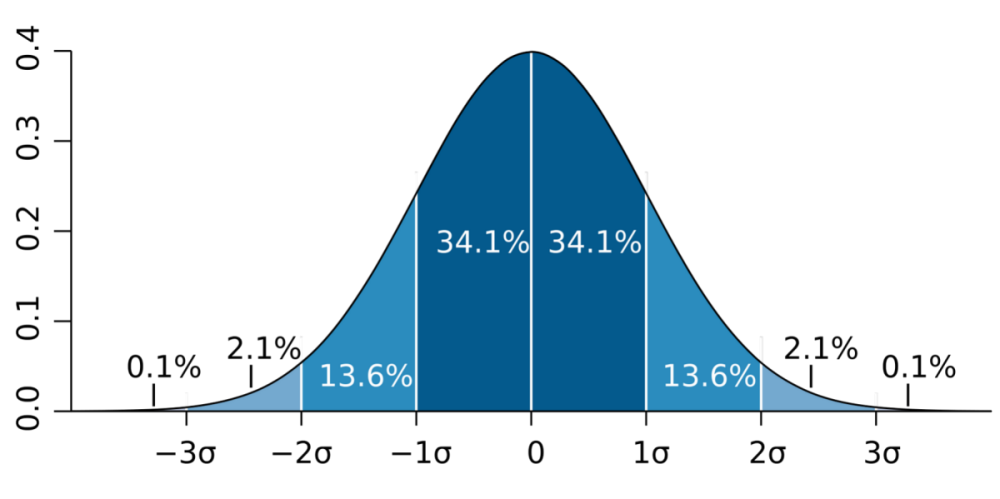
\includegraphics[width=0.85\textwidth]{normal.distribution.png}
                %        \caption{}
            \end{figure}
        \end{column}

        \begin{column}{0.40\textwidth}
            \begin{equation}
                \large
                p(x) = \frac{1}{\sigma\sqrt{2\pi}} \; e^{-\frac{1}{2}(\frac{x-\mu}{\sigma})^2}
            \end{equation}
        \end{column}

    \end{columns}
\end{frame}


\begin{frame}{}
    \begin{figure}
        \centering
        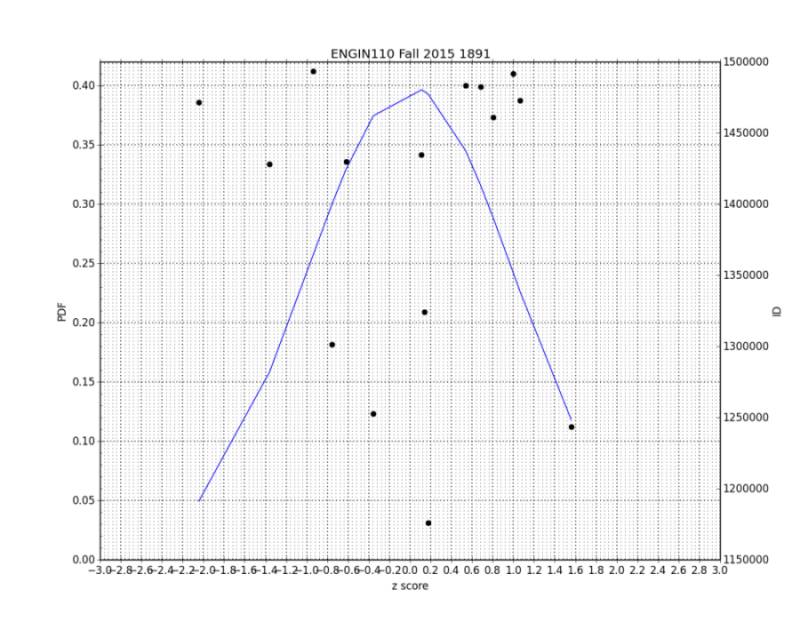
\includegraphics[width=0.80\textwidth]{class.png}
%        \caption{}
    \end{figure}
\end{frame}


\begin{frame}[plain]{}
    \centering\LARGE\textbf{Likelihood}
\end{frame}


\addtocounter{framenumber}{-1}
\begin{frame}{\href{https://uidaho.pressbooks.pub/riskassessment/chapter/likelihood/}{Likelihood} is a tool for summarizing the data’s evidence about unknown parameters}
    \begin{enumerate}[series=outerlist,topsep=0pt,itemsep=3pt,leftmargin=*,label=(\arabic*)]
        \item[]Normal distribution depends on two parameters
    \end{enumerate}

    \vspace*{\fill}

    \begin{equation}
        \Large
        f(x;\mu,\sigma) = \frac{1}{\sigma\sqrt{2\pi}} e^{-\frac{(x-\mu)^2}{2\sigma^2}}
    \end{equation}

    \vspace*{\fill}

    \begin{enumerate}[series=outerlist,topsep=0pt,itemsep=11pt,leftmargin=*,label=(\arabic*)]
        \item[] $f$ -- \acs{pdf} when the parameters are constant and we vary in $x$
        \item[] $f$ -- likelihood when $x$ is constant and the parameters vary
    \end{enumerate}

    \vspace*{\fill}

    \begin{enumerate}[series=outerlist,topsep=0pt,itemsep=11pt,leftmargin=*,label=(\arabic*)]
        \item[]A common application of the likelihood function is in estimation
        \item[]Estimate parameters from some given data $x$ to understand how the function behaves if it has `fat tails' or really skewed
    \end{enumerate}
\end{frame}


\begin{frame}{There may not be a lot of data where the true mean, etc., could be directly obtained}
    \begin{enumerate}[series=outerlist,topsep=0pt,itemsep=15pt,leftmargin=*,label=(\arabic*)]
        \item[]Example of statistical inference
        \item[]If a coin is `fair' then we know $p = 0.5$ and can use the binomial distribution for the \acs{pdf}
    \end{enumerate}

    \vspace*{\fill}

    \begin{equation}
        \LARGE
        f(x) = \frac{n!}{x!(n-x)!}p^x(1-p)^{(n-x)}
    \end{equation}

    \vspace*{\fill}

    \begin{enumerate}[series=outerlist,topsep=0pt,itemsep=15pt,leftmargin=*,label=(\arabic*)]
        \item[]For 10 flips of the fair coin --
    \end{enumerate}

    \vspace*{\fill}

    \begin{equation}
        \LARGE
        f(x;p) = \binom{10}{x}0.5^x(1-0.5)^{(10-x)}
    \end{equation}
\end{frame}


\begin{frame}{What if you don't know the coin is fair?}
    \begin{enumerate}[series=outerlist,topsep=0pt,itemsep=21pt,leftmargin=*,label=(\arabic*)]
        \item[]You see 7 heads on 10 flips
        \item[]Now it's a likelihood function
    \end{enumerate}

    \vspace*{\fill}

    \begin{equation}
        \LARGE
        L(p;x) = \binom{10}{7}p^7(1-p)^3
    \end{equation}

    \vspace*{\fill}

    \begin{enumerate}[series=outerlist,topsep=0pt,itemsep=15pt,leftmargin=*,label=(\arabic*)]
        \item[]Typically to find p, find the maximum or log maximum
    \end{enumerate}
\end{frame}


\begin{frame}{}
    \begin{figure}
        \centering
        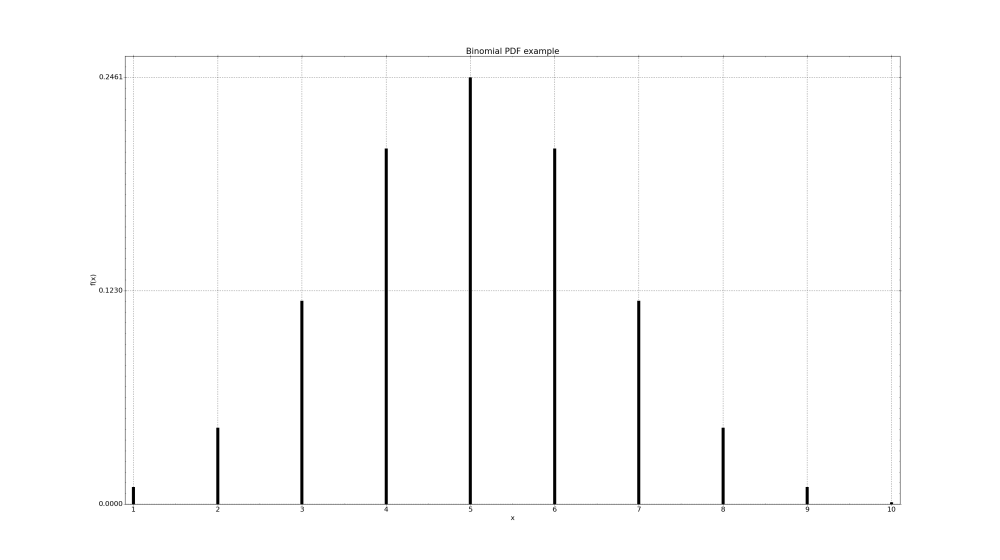
\includegraphics[width=0.90\textwidth]{binomial.pdf.png}
%        \caption{}
    \end{figure}
\end{frame}


\begin{frame}[plain]{}
    \centering\LARGE\textbf{Statistics critique}
\end{frame}


\addtocounter{framenumber}{-1}
\begin{frame}{Statistics get a bad rap}
    \begin{quote}
        There are three kinds of lies:  lies, damned lies, and statistics.\\
        --Benjamin Disraeli
    \end{quote}

    \vspace{0.25in}

    \begin{quote}
        I gather, young man, that you wish to be a Member of Parliament. The first lesson that you must learn is, when I call for statistics about the rate of infant mortality, what I want is proof that fewer babies died when I was Prime Minister than when anyone else was!\\
        --Winston Churchill
    \end{quote}
\end{frame}


\begin{frame}{}
    \begin{figure}
        \centering
        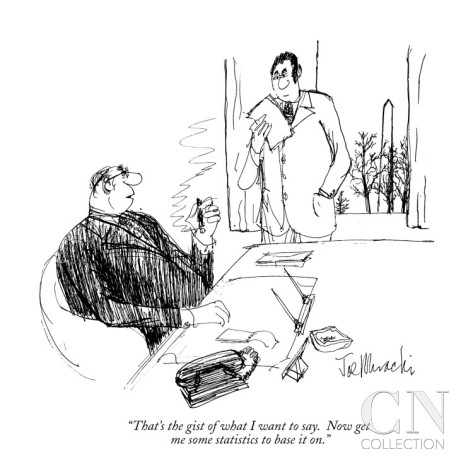
\includegraphics[width=0.55\textwidth]{cartoon.jpg}
%        \caption{}
    \end{figure}
\end{frame}


\begin{frame}{Statistics are tools, not ends}
    \begin{quote}
        It is very easy for research psychologists, particularly young psychologists, to be overconcerned with statistical methods\ldots\\
        However, \textbf{careful observation} is the main business of empirical science, and statistical methods are useful only so long as they help, not hinder, the \textbf{systematic exploration of data} and the accumulation and coordination of results.\\
        --William Hays (1963)
    \end{quote}
\end{frame}


\begin{frame}{Statistical inference -- The `grand thing of reasoning backwards'}
    \begin{quote}
        In solving a problem of this sort, the grand thing is to be able to reason backward. That is a very useful accomplishment, and a very easy one, but people do not practise it much...Most people, if you describe a train of events to them, will tell you what the result would be.\\
        They can put those events together in their minds, and argue from them that something will come to pass.  There are few people, however, who, if you told them a result, would be able to evolve from their own inner consciousness what the steps were which led up to that result.\\
        This power is what I mean when I talk of reasoning backwards\ldots\\
        --Sherlock Holmes, A Study in Scarlet
    \end{quote}
\end{frame}


\begin{frame}[plain]{}
    \centering\LARGE\textbf{Let's look at some \href{https://uidaho.pressbooks.pub/riskassessment/chapter/probability-and-statistics/}{seminal cases}}
\end{frame}


\begin{frame}[plain]{}
    \centering\LARGE\textbf{Cholera}
\end{frame}


\addtocounter{framenumber}{-2}
\begin{frame}{In 1854, there was a cholera outbreak near Broad Street in London}
    \begin{enumerate}[series=outerlist,topsep=0pt,itemsep=3pt,leftmargin=*,label=(\arabic*)]
        \item[]Over 500 people died
        \item[]Seminal epidemiological study by Dr. John Snow
        \item[]They did not know cholera was water borne
            \vspace{0.10in}
        \item[]\textbf{Snow knew nothing at the time!}
            \vspace{0.10in}
        \item[]Snow mapped the 13 public wells and known cholera deaths (Soho)
        \item[]Not great water treatment practices back then
        \item[]Spatial clustering of cases around one particular water pump  
        \item[]SW corner of Broad Street and Cambridge Street  
        \item[]Others died who had water delivered from that pump  
        \item[]Or went to school there
            \vspace{0.10in}
        \item[]Shut it down and new cases stopped
    \end{enumerate}
\end{frame}


\begin{frame}{}
    \begin{figure}
        \centering
        
\includegraphics[width=0.85\textwidth]{snow.png}
%        \caption{}
    \end{figure}
\end{frame}


\begin{frame}{}
    \begin{figure}
        \centering
        
\includegraphics[width=0.85\textwidth]{walker.jpg}
%        \caption{}
    \end{figure}
\end{frame}


\begin{frame}[plain]{}
    \centering\LARGE\textbf{WWII}
\end{frame}


\addtocounter{framenumber}{-1}
\begin{frame}{Statistics is even used in war}
    \begin{enumerate}[series=outerlist,topsep=0pt,itemsep=21pt,leftmargin=*,label=(\arabic*)]
        \item[]Too many Allied planes were getting shot down over Germany
        \item[]During WWII, statistician Abraham Wald was asked to catalog the location of bullet holes on returning Allied aircraft and determine the best places to reinforce the planes with armor
        \item[]To reduce losses
        \item[]Take observations of planes that did return
        \item[]Draw map of where each aircraft was hit (generally)
    \end{enumerate}
\end{frame}


\begin{frame}{}
    \begin{figure}
        \centering
        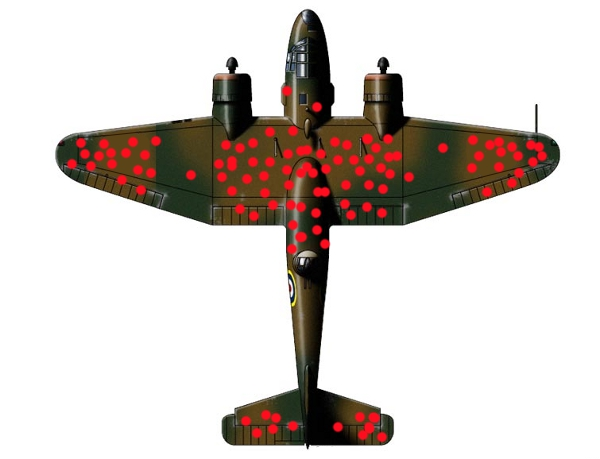
\includegraphics[width=0.80\textwidth]{wwii.plane.jpg}
%        \caption{}
    \end{figure}
\end{frame}


\begin{frame}{}
    \begin{figure}
        \centering
        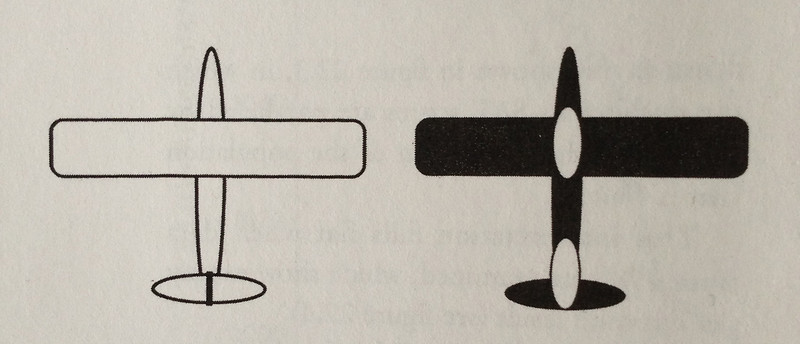
\includegraphics[width=0.85\textwidth]{wwii.planes.jpg}
%        \caption{}
    \end{figure}
\end{frame}


\begin{frame}{Wald's supervisors concluded that nose, wings, fuselage were covered in damage and needed more armor}
    \begin{enumerate}[series=outerlist,topsep=0pt,itemsep=21pt,leftmargin=*,label=(\arabic*)]
        \item[]Wald said, no
        \item[]Why?
        \item[]He recognized survivorship bias in the sample
        \item[]Allies were only sampling planes that completed their missions and returned home
        \item[]A form of sampling bias
    \end{enumerate}
\end{frame}


\begin{frame}{Don't miss the forest for the trees when analyzing tons of data}
    \begin{enumerate}[series=outerlist,topsep=0pt,itemsep=21pt,leftmargin=*,label=(\arabic*)]
        \item[]Garbage in = garbage out
        \item[]Good data in != good conclusions out without good analysis -- Engineering judgement
        \item[]And that applies to risk assessment how?  
        \item[]When we were critisizing utilitarianism
    \end{enumerate}
\end{frame}


\begin{frame}[plain]{}
    \centering\LARGE\textbf{Challenger}
\end{frame}


\addtocounter{framenumber}{-1}
\begin{frame}{The Challenger explosion was the first space shuttle catastrophe}
    \begin{enumerate}[series=outerlist,topsep=0pt,itemsep=11pt,leftmargin=*,label=(\arabic*)]
        \item[]28 January 1986  
        \item[]Forecast calls for abnormally low temperature (30\degree F)   
        \item[]Engineers recommend against launch due to concern about O-ring failure
        \item[]NASA flight control overrules  
        \item[]O-rings had failed due to cold temperatures on the morning of the launch  
        \item[]Challenger explodes shortly after launch (73 seconds)  
        \item[]First time this happened  
        \item[]Christa McAuliffe, teacher from New Hampshire, selected to teach lessons from space
        \item[]This was a big deal leading up to the launch
    \end{enumerate}
\end{frame}


\begin{frame}{Launch was already delayed for six days due to weather, technical problems}
    \begin{enumerate}[series=outerlist,topsep=0pt,itemsep=21pt,leftmargin=*,label=(\arabic*)]
        \item[]Reagan appointed a special commission to determine what went wrong with Challenger and to develop future corrective measures  
        \item[]Neil Armstrong and Chuck Yeager on the commission
        \item[]O-ring seal on solid rocket booster became brittle  
        \item[]Flames broke out and damaged the external fuel tank  
        \item[]NASA managers were aware of these design problems but also failed to act  
        \item[](Lack of ethical context)
    \end{enumerate}
\end{frame}


\begin{frame}{Launches resumed in 1988 after redesigns}
    \begin{enumerate}[series=outerlist,topsep=0pt,itemsep=21pt,leftmargin=*,label=(\arabic*)]
        \item[]But there still have been failures  
        \item[]Would there ever be 100\% safety?
        \item[]Are there more contemporary analogues?
    \end{enumerate}
\end{frame}


\begin{frame}{\href{https://uidaho.pressbooks.pub/riskassessment/chapter/contemporary-cases-in-risk-assessment-2/}{Lessons learned from the Space Shuttle Challenger}}
    \begin{enumerate}[series=outerlist,topsep=0pt,itemsep=15pt,leftmargin=*,label=(\arabic*)]
        \item[]Argue that the very concept of risk management must be called into question  
        \item[]Using a failure modes effects analysis without any quantitative risk measures
        \item[]Bad analysis to determine catastrophic mission failure
        \item[]Astronauts were completely unaware of the specific dangers that the O-rings pose  
        \item[]Did not give an \textbf{informed consent} to launch
        \item[]O-ring design ranked fourth out of four submitted engineering designs
        \item[]Everything in the area of risk management is a matter of ethics
    \end{enumerate}
\end{frame}


\begin{frame}[plain]{}
    \centering\textbf{Was it necessary to take cavalier chances with risky technology in order to make progress in the arena of space exploration?}
\end{frame}


\addtocounter{framenumber}{-1}
\begin{frame}{}
    \begin{columns}[c]

        \begin{column}{0.65\textwidth}
            \begin{figure}
                \centering
                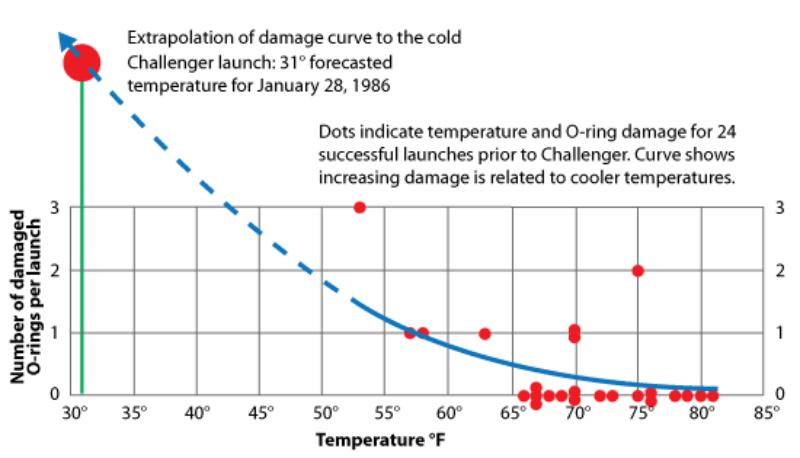
\includegraphics[width=0.95\textwidth]{challenger.jpg}
                %        \caption{}
            \end{figure}
        \end{column}

        \begin{column}{0.35\textwidth}
            \begin{enumerate}[series=outerlist,topsep=0pt,itemsep=15pt,leftmargin=*,label=(\arabic*)]
                \item[]Initial analysis did not include mission with 0 damage  
                \item[]Trend was not observed
                \item[]3 incidents of thermal distress occurred out of twenty flights at 66\degree F or greater
            \end{enumerate}
        \end{column}

    \end{columns}
\end{frame}


\begin{frame}{}
    \begin{columns}[c]

        \begin{column}{0.65\textwidth}
            \begin{figure}
                \centering
                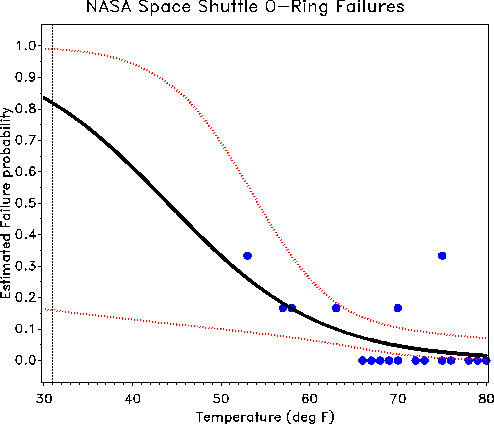
\includegraphics[width=0.95\textwidth]{challenger.prob.jpg}
                %        \caption{}
            \end{figure}
        \end{column}

        \begin{column}{0.35\textwidth}
            \begin{enumerate}[series=outerlist,topsep=0pt,itemsep=15pt,leftmargin=*,label=(\arabic*)]
                \item[]4 \textbf{flights} at 63\degree F or below experienced thermal distress
                \item[]Probability of O-ring distress is increased to almost a certainty if the temperature of the joint is less than 65\degree F
            \end{enumerate}
        \end{column}

    \end{columns}
\end{frame}


\begin{frame}[plain]{}
    \centering\LARGE\textbf{Misconceptions}
\end{frame}


\addtocounter{framenumber}{-1}
\begin{frame}{These case studies point to common misconceptions about the use of statistics}
    \begin{enumerate}[series=outerlist,topsep=0pt,itemsep=3pt,leftmargin=*,label=(\arabic*)]
        \item[]\textbf{Statistics is mostly mathematics, formulas, proofs}
        \item[]Statistics is the science of data, their production, how to make the right inferences
            \vspace{0.25in}
        \item[]\textbf{Statistics is obvious}
        \item[]Statistical inference can be highly counterintuitive and often involves `backwards reasoning'
            \vspace{0.25in}
        \item[]\textbf{Statistical analyses can easily be done by computers}
        \item[]Nothing relieves the investigator of the direct responsibility of understanding data and how best to analyze and interpret
    \end{enumerate}
\end{frame}


\begin{frame}{I don’t plan on doing research myself, I just want to learn interesting things about\ldots}
    \begin{enumerate}[series=outerlist,topsep=0pt,itemsep=21pt,leftmargin=*,label=(\arabic*)]
        \item[]Engaging in science at any level (including as a consumer) requires critical analysis
        \item[]Knowledge of statistical methods is needed to protect us against false claims, junk science
    \end{enumerate}
\end{frame}


\begin{frame}[plain]{}
    \begin{figure}
        \centering
        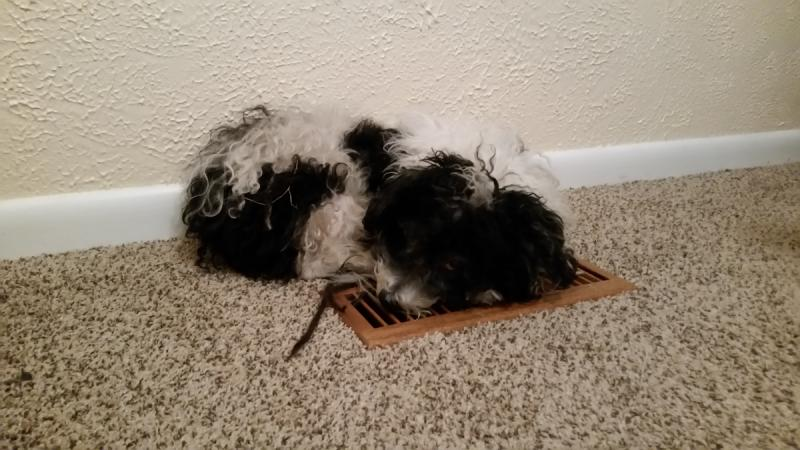
\includegraphics[width=0.65\textwidth]{final.jpg}
%        \caption{}
    \end{figure}
\end{frame}


%%%%%%%
%\begin{frame}{}
%    \begin{columns}
%
%        \begin{column}{0.50\textwidth}
%            \begin{enumerate}[series=outerlist,topsep=0pt,itemsep=21pt,leftmargin=*,label=(\arabic*)]
%                \item[]
%                \item[]
%            \end{enumerate}
%        \end{column}
%
%        \begin{column}{0.50\textwidth}
%            \begin{enumerate}[series=outerlist,topsep=0pt,itemsep=21pt,leftmargin=*,label=(\arabic*)]
%                \item[]
%                \item[]
%            \end{enumerate}
%        \end{column}
%
%    \end{columns}
%\end{frame}

%    \begin{figure}
%        \centering
%        \includegraphics[width=0.75\textwidth]{wsc.png}
%        \caption{\acs{wsc}}
%    \end{figure}


%\begin{frame}{References}
%    \bibliographystyle{nsf}
%    \footnotesize
%    \bibliography{references}
%\end{frame}
%%%%%%%


\end{document}
